\chapter{Methods}
\label{chp:data}

\section{Data Acquisition}
Eclipsing binary optical data acquisition requires an observer to do time series ccd photometry
of one target with an observation cadence dependent on the period of the system.
For example, the data gathered for this project was collected on multiple nights and observed on the order of hours with evenly timed frames.

\subsection{Planning Observations}
There are some options for selecting sources to observe.
The following process is one learned in practice with amateur astronomer Carlos Colazo of Argentina.
This study uses the Variable Star and Exoplanet Section of Czech Astronomical Society's observation project called
BRNO Regional Network of Observers (BRNO)~\cite{brno}.

An ephemeris is made by using a table of predicted times of minima published on the BRNO webpage.
For site specific predictions, the webpage needs to be visited in the original Czech language.
A web form shown in figure~\ref{fig:brno} appears to include latitude and ELongitude (longitude in degrees east of the meridian) of the observation site.
\begin{figure}[h]
    \centering
    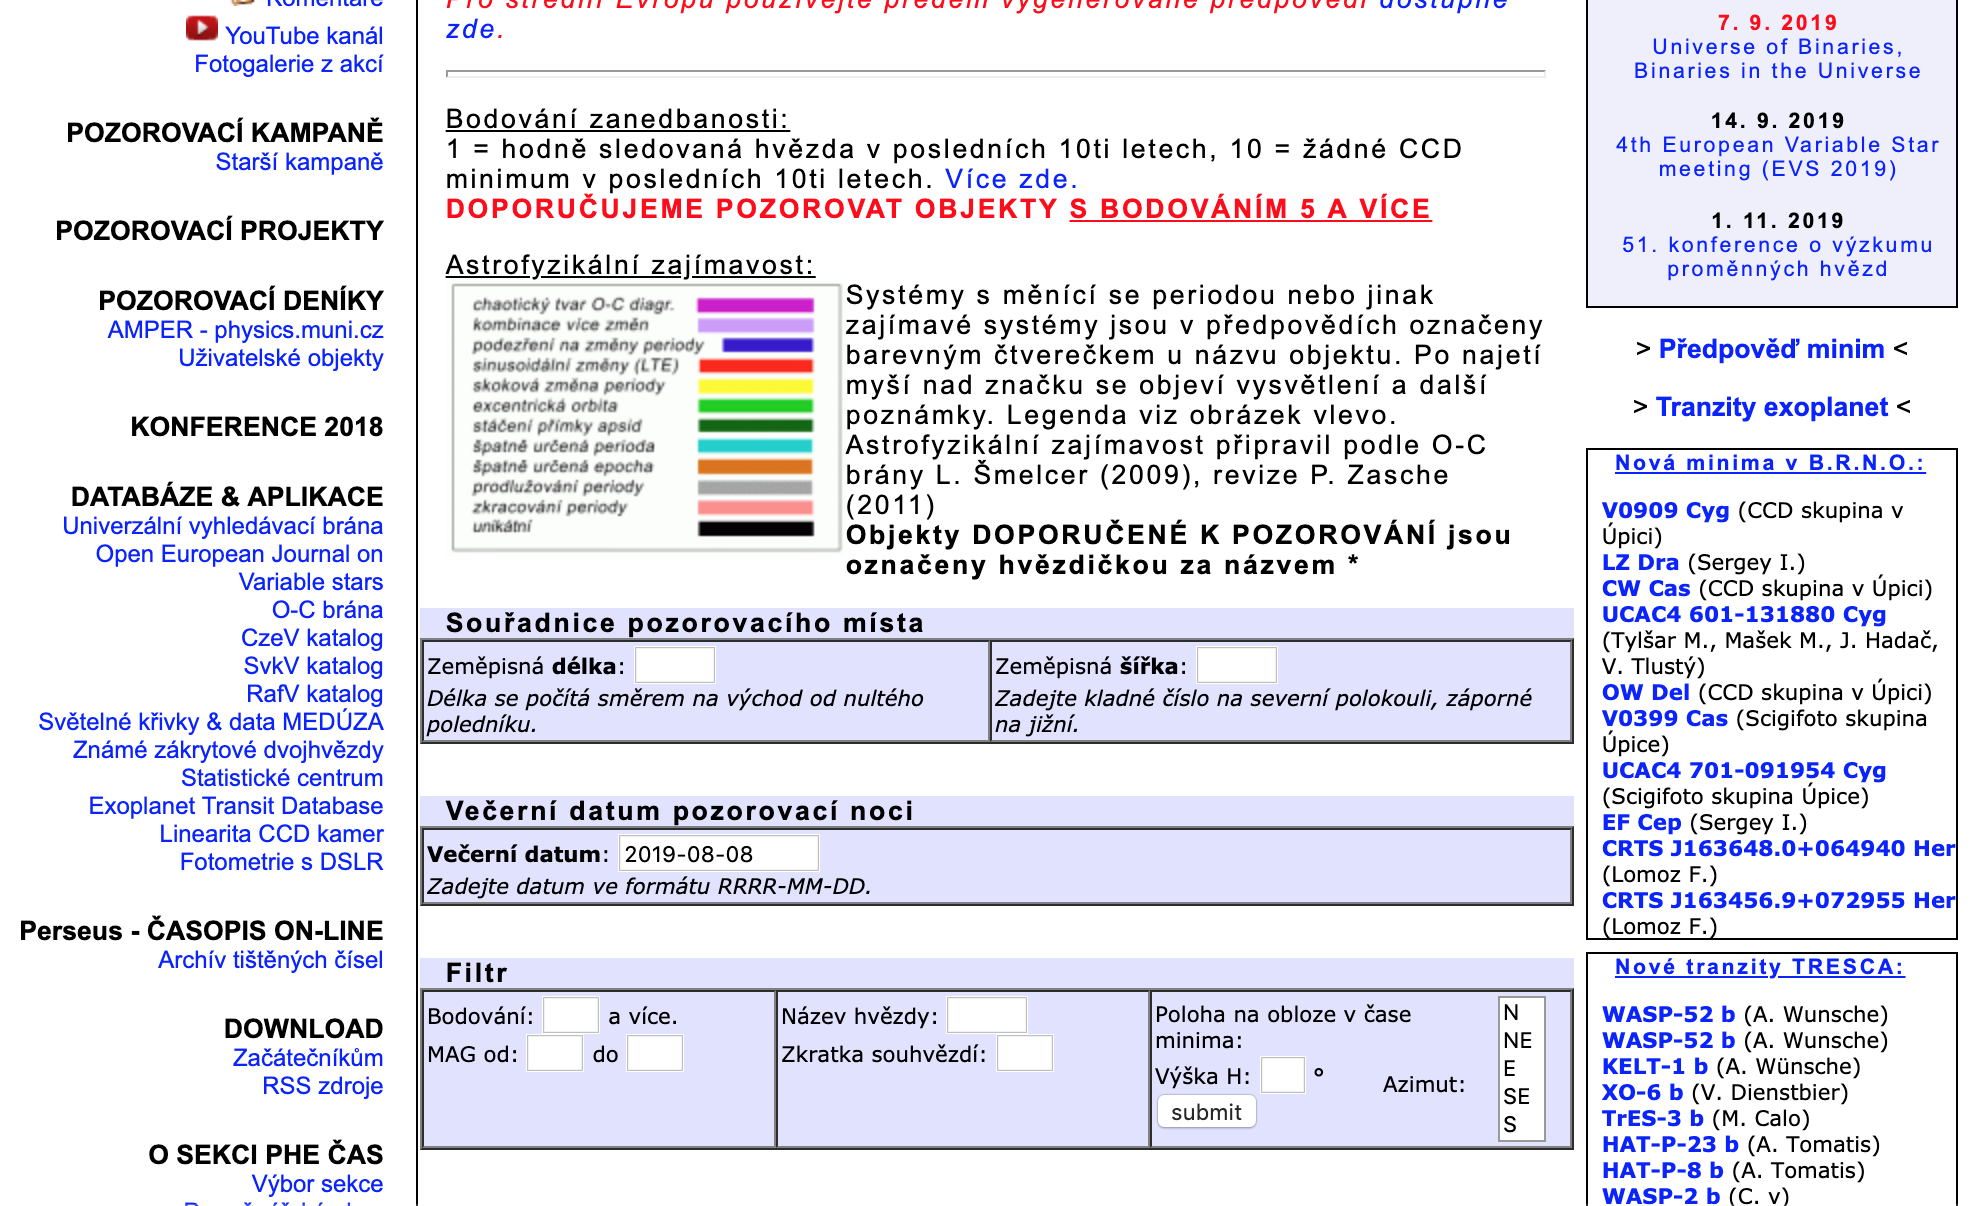
\includegraphics[width=\columnwidth]{figures/brno.png}
    \caption{Web form for eclipsing binary predicted times of minima from the Variable Star and Exoplanet Section of Czech Astronomical Society's observation project called BRNO Regional Network of Observers (BRNO)}
\label{fig:brno}
\end{figure}

It is important to mention the American Association of Variable Star Observers (AAVSO)
offers a target tool on the web~\footnote{\url{https://filtergraph.com/aavso}} to help make an observation plan.


\subsubsection{Selection criteria}
Typically, EW type binary stars have the shortest period and were chosen for this reason. 
Observation time is set to start no later than one hour before the predicted time of minima.
The error on the predicted time of minima can be great due to lack of observational data.

BRNO classifies stars using a scale from 1 to 10.
As a rule of thumb, the scale refers to the number of years since last reported observation.
BRNO explicitly recommends observers observe objects with a rating of 5 or more.

Since observation are made over several hours it is best practice to pick objects on the eastern parts of the sky.
This allows for maximum viewing time. The altitude of the target should be above 30 degrees for proper photometry study, but 
can be slightly lower.

Lastly, as with all observations, the limiting magnitude of the system will dictate what objects are observable.
The change in magnitude of known eclipsing binaries stated in catalogs.
The observer must make certain that the instrumentation allows for such observation.
Millimagnitude precision is standard in exoplanet research, but is not required for any of the observations in this study.

\subsection{Observation}
When performing an eclipsing binary observation the observer should attempt to observe 
the same binary system through the entire night to capture the most complete period. 
Some systems need to be observed across several nights to obtain a full period.
When conducting any measurement it is good practice to make plots on-the-fly to make sure the quality of data is consistent.

Since the observer typically will begin observation on the eastern sky with a low altitude, the air mass will be highest
at the beginning of the observation.
This can present a problem if the observer does not consider the increase of flux as the object approaches zenith or the highest
point in the sky.
When the object being observed reaches zenith, the air mass is the lowest and if not considered can cause over saturation of the CCD\@.
Saturation is when the potential well for the pixel is completely filled and will no longer capture the electrons
converted from the photon interaction with the CCD\@.

\subsection{Post observation}
After the observation is complete it is vital to collect calibration frames required for proper data reduction for photometry.
Data reduction is the process for removing noise due to dark current, bias, and any obscuring defects in the optical path of the system.
Required calibration frames are,
\begin{description}
    \item[Flat Frames] Flat frames are made by using an evenly illuminated light source. This can be created by using a white screen
        and a diffuse white light. This process will show any obscuring defects that are in the optical path like dust and vignetting.
        The required exposure time depends on the lighting system to reach a signal between 30 to 50 percent of saturation.
    \item[Dark Frames] Dark frames are made by taking closed `exposures' of the CCD\@. Exposure time for the dark frames need to match
        the flat frame exposure times and object exposure times.
    \item[Bias Frames] Bias frames are only needed if the observer does not match the dark frame exposure times to the flat frames. 
        To take bias frames, the observer must take the shortest allowed exposure. Depending on software, by selecting the type of frame as bias,
        the exposure time will automatically be adjusted or displayed as zero.
\end{description}

\section{Motivation for pipeline: lightcurator}
Observing eclipsing binary systems especially of EW type require an observer to track the source on the order of hours.
This means the data produced can include various stars as well as some potentially undiscovered variable stars.
For this reason, the author created a python package called 
\textit{lightcurator}~\cite{castillo_2019} which is publicly available on Github \url{https://github.com/moemyself3/lightcurator}
and on PyPI \url{https://pypi.org/project/lightcurator/} for easy installation using the package insaller for Python, \textit{pip}.
Lightcurator includes 2 packages: \textit{lightcurve} and \textit{calibration}.
The functions included are described in the sections that follow.
Future plans are documented as GitHub Issues and labeled
as Enhancements~\footnote{The reader is encouraged to contribute to Enhancements and create pull requests.}.

\section{Pipeline for variable star detection}
\begin{enumerate}
    \item Reduce data
    \item Align frames
    \item Create deepsky frame
    \item Plate solve deepsky
    \item Scrape deepsky header and add WCS to aligned frames
    \item Extract sources from aligned frames
    \item Extract sources from deepsky frame
    \item Cross match sources from aligned frames to deepsky frame
    \item Cross match master catalog with catalogs like VSX and GCVS
    \item Correct or normalize extracted flux data
    \item Create or update database of previously observed sources
    \item Plot individual light curves
    \item Analyze individual light curves for variability estimation
    \item Sort database given variability ranking
\end{enumerate}

\subsection{Data reduction}
Reading, writing fits files, and creating data tables is done with a python
package called \textit{astropy}~\cite{astropy_2013,astropy_2018}.
Majority of the data reduction is done with astropy core package,
coordinated packages, and affiliated packages.
Coordinated packages are maintained by the Astropy Project
and affiliated packages are not maintained by the Astropy Project,
but is a part of the Astropy Project community.

Coordinated packages in use are \textit{astroquery}~\cite{astroquery}, \textit{ccdproc}~\cite{ccdproc}, \textit{photutils}~\cite{photutils}.
An affiliated package in use is \textit{astroscrappy}~\cite{astroscrappy}.
A package in the process of becoming an official affiliated package that is in use is \textit{astroalign}. 
More details of astroalign are discussed in Section~\ref{section:align} 

\subsubsection{Calibration}
Lightcurator has a module called calibration that provides the tools for convenient data reduction.
The routine begins with the creating of the list of the fits files to be used
with \textit{ccdproc.ImageFileCollection}.
The list is used for quick reference to all the fits files to be processed.
The \textit{validate\_units} function checks for the fits keyword `BUNIT'. 
If the units are missing then the function raises an exception and suggests
to the user to use the \textit{add\_units} function. 
All the data sets including flats and darks collected at CTMO are missing units.
This function inserts the `BUNIT' keyword and sets the value to `adu'.

After defining the paths to the location of the calibration files, i.e.\
flats and darks, running \textit{create\_masters} makes a master dark and master flat frame.
This is done by doing a median combine of the dark frames. 
The dark frames are a measure of dark current which is the noise generated by the thermal energy generated by the silicon of the CCD\@.
Since the CCD has a constant voltage applied across the device, there is a bias in the signal generated that contains some read noise.
By taking dark frames at the same exposure time as flat frames bias frames can be ignored since the noise will also be removed along
with the dark frame.

The function \textit{reduce} takes a user defined read noise, gain, and
path to the directory containing the data to be reduced. 
The \textit{reduce} function gain corrects the master dark and master flat then
uses \textit{ccdproc.ccd\_process}. 
The \textit{ccdproc.ccd\_process } is an all-in-one function that gain corrects,
dark subtracts, and flat corrects. It can also take into considerations 
uncertainties for error propagation, over scan regions, and any trimming that
may be required in different set ups.
The new reduced fits frames are then saved to file for later processing.

Through this process it is important to note that the file goes from storing
16-bit data to 64-bit data.
This can easily cause a significant impact on a systems storage
since the new frames are about 4 times larger than before.

\subsubsection{Cosmic ray detection}
It is not uncommon to have cosmic rays hit the CCD causing peaks in signals that may be confused as sources during source extraction.
The final step in data reduction is cosmic ray detection.
For this, the function \textit{ccdproc.cosmicray\_lacosmic} identifies cosmic rays by identifying pixels based on a variation of
Laplacian edge detection described by van Dokkum~\cite{lacosmic} and implemented by McCully in \textit{astroscrappy}~\cite{astroscrappy}.
Lightcurator uses this algorithm with a function called \textit{hotpixfix} prior to alignment of frames to allow a flexible
approach by using raw frames instead of properly reduced frames.

\subsection{Align frames}
\label{section:align}
Frame alignment is done with a python package called \textit{astroalign} written by Dr.\ Martin Beroiz~\cite{beroiz_2019} which is publicly
available on Github\footnote{For the latest version of astroalign check: \url{https://github.com/toros-astro/astroalign}}

Astroalign is the preferred method for image alignment since the raw data frames do not have World Coordinate System (WCS) information attached to
the headers.
WCS information encodes the transformations required to change $x,y$-pixel location to right ascension (RA) and declination (DEC).

Lightcurator uses a function called \textit{try\_register} to catch exceptions and reject by truncating the data frame if alignment
cannot be completed.
Exceptions from astroalign that are most commonly experienced are \textit{MaxIterError} which is raised when the maximum number of iterations
allowed by astroalign are met and a custom \textit{Exception} raised when there are less than 3 sources detected.

Lightcurator assumes that there may be drift though the entire series of
frames.
For this reason, the frame in the middle of the time series is taken as the
reference image.

\subsection{Create deepsky frame}
To create a deepsky frame a simple addition of all aligned frames are made.
The CCD data is loaded into python as CCDData or numpy.ndarray types.
Simple addition is used since the deepsky frame is only used for source 
detection and not for photometry.
A more appropriate method for combining frames for photometry would 
be a median combine. 
This is not performed in this step since calculating the median would require
more processing time and memory.

\subsection{Plate solve deepsky}
Plate solving is the process in which the exact position of the field
is found by matching indexed data with the relative positions of the
sources on the field in question.

Astrometery.net~\cite{lang_2010} is a service that exists online
and as a standalone program that can solve the astrometry of a field.

Lightcurator acts as a wrapper that calls on the processes 
\textit{solve-field} from astrometry.net.
This starts the blind astrometric solving.
If the fits header contained pointing information such as RA/DEC, then
the solving process could be directed where to start the search for matching.
Since no information was directly available from the header file blind solving
was required.
The initial search starts very wide and could take up to 30 
minutes~\footnote{The user can choose a timeout parameter to
stop the process after a certain amount of time.} if there are
very few sources in the field.

\subsection{Scrape deepsky header and add WCS to aligned frames}
Using Astropy's fits and WCS tools, lightcurator reads the header copies the 
WCS from the deepsky frame that was plate solved with Astrometer.net's service.
Up to this point, the headers of all the aligned frames are blank.
We attach WCS information and the keyword and value assigned to `DATE-OBS' which
is the time stamp of the observation.


\subsection{Source Extraction}
Source extraction is done with a python package called \textit{photutils}.
The steps to source extraction are as follows.
First, an Astropy.stats function called \textit{sigma\_clipped\_stats} takes
        the data frame finds the standard deviation, $\sigma$,
        and the median. Then, all points smaller or larger than $3 \sigma$
        from the median are removed or clipped.
        This step is done repeatedly 
        until there are no more points beyond $3 \sigma$ or 5 cycles have
        been completed. Lightcurator has hard-coded $3 \sigma$ and the 
        maximum iterations of 5. The function returns 
        the calculated clipped $\sigma$, mean, and median.

From photutils, the class \textit{DAOStarFinder}
uses the DAOFIND algorithm developed
by Stetson in 1987~\cite{stetson_1987}. 
Lightcurator hard-codes the full width half max (fwhm)
at 3.0 and detection threshold at $5 \sigma$ 
above the background.
DAOFIND returns a method to find stars. 
The data is background subtracted before the \textit{find\_stars} method
is called.
The background is the median calculated in the first step.
The method returns a table containing an id, xy centroid, instrumental
flux, and instrumental magnitude on the stars found.

This method is applied to each aligned frame to create a catalog
of sources for each frame.
Lightcurator refers to these as aligned cats.

\subsection{Extract sources from deepsky frame}
The same method described in the previous section is done to the
deepsky frame to create a master catalog of all
possible sources detected in the frame.

\subsection{Cross match sources from aligned frames to deepsky frame}
Source cross matching is done with an Astropy package
called \textit{coordinates} using the \textit{SkyCoord} class.
The aligned catalogs are then compared to the master catalog one at a time. 
The SkyCoord class creates a method called \textit{match\_to\_catalog\_sky}
which finds the nearest coordinate match between each 
object of the two catalogs.
The matched catalog contains the same information from the sources, but
only from those sources that best matched coordinates.
The matched catalogs are written to file.

The final step in cross matching catalogs is to create a time series
catalog that contains the id of all the sources, their fluxes, and 
time stamp from the observation.
This is written to file and saved as an ecsv file by recommendation
of Astropy documentation.

\subsection{Cross match master catalog with other catalogs}
The lightcurator function \textit{query\_from\_wcs} takes a string path
to a fits file with WCS\@.
The function expects the header keywords specific to WCS
information `CRVAL1' and `CRVAL2' for RA and DEC, respectively.
Using \textit{query\_region} from the astroquery package, a search cone of 30 arc minutes is generated
from a Vizier query of the following catalogs,
\begin{description}
    \item[B/vsx] AAVSO International Variable Star Index VSX~\cite{vsx}, 
    \item[B/gcvs] General Catalogue of Variable Stars~\cite{samus_2017},
    \item[I/340] UCAC5 Catalogue~\cite{ucac5},
    \item[I/345] Gaia DR2~\cite{gaia2}.
\end{description}

A similar process as described in the previous section is used to match
the master catalog with the Vizier query.
At this point, the user can verify that the intended eclipsing binary 
star system is in both VSX and GCVS catalogs and that the index
from both query results match with each other.
The query results are used as an intermediary step, therefore only stored to memory.
The reported magnitudes from UCAC and Gaia use standard filters and can be used to calibrate instrumental data.


\subsection{Correct or normalize extracted flux data}
Calibration stars are required to transform instrumental
flux measurements from filtered data to a standard magnitude system.
This is usually done by using cataloged magnitudes the report in a standard set of filters like Johnson UVBRI or Sloan ugriz. 
Since most data is unfiltered, the observations are long with changing
air mass, and the field of view is small, differential photometry is used.

Differential photometry uses comparison stars to remove the effects of
extinction due to changing air mass.
Comparison stars are found using the following criteria, 
\begin{enumerate}
    \item the star must not be a variable star,
    \item the stars must be about the same magnitude,
    \item the standard deviation of the star must not be too large, and
    \item the star needs to be visible for most of the observation.
\end{enumerate}

Lightcurator does not yet have the tool implemented for finding comparison stars, but is under development.
To meet criteria 1 a filter is generated by using the list returned from
the matched sources to the VSX and GCVS catalog.
Criteria 3 is met by running numpy statistics that calculate standard deviation that ignores \textit{nan} values.
Criteria 4 is met by counting the \textit{nan} values across the time series of a single source and filtering
sources with a count less than an arbitrary tolerance set at 10 percent. 
Criteria 4 is done by visual inspection.

The average magnitude of the comparison stars is taken for a single frame.
The averaged magnitude is subtracted from the magnitude of the variable star.
This is done across all frames in the time series catalog.
The features due to changing air mass would appear on both variable and 
comparison stars.
By subtracting the magnitude of the comparison star from the
variable star, the variability of the star will become apparent. 
The difference of a non-variable star to the magnitude of the comparison
will reveal a horizontal plot, if comparison stars meet the criteria. 

\subsection{Create or update database of previously observed sources}
The database is not yet implemented in lightcurator, but is intended to 
provide magnitudes from previous observations processed by lightcurator.
Tracking sources in this way will enable analysis for longer period variable stars.
Future plans for lightcurator include to allow users to upload their own time series data into the database and
to make a streamable service that can update the database of previously observed sources with data from new single
frames to update light curves.

\subsection{Analyzing variability}
Currently, lightcurator only identifies variable stars using catalog
matching with VSX and GCVS\@. 

Immediate plans for variability analysis will be done with a python package 
called feets: feATURE eXTRACTOR FOR tIME sERIES,
written by Cabral~\cite{cabral_2018}.

\section{Eclipsing binary system modeling}
PHOEBE~\cite{prsa_2005, prsa_2016, horvat_2018} provides tools to create a mesh for detached, semi-detached, and contact binary stars.
First, a system needs to be created that will contain all the parameters of the objects studied.
Light curve data, i.e.\ magnitude and time, is imported to the parameter list.
This step would also include importing orbital, effective temperature, and radial velocity information.
When setting up the system PHOEBE automatically provides defaults to only require magnitude and time as inputs.
For this process a close contact binary system is setup since the type of stars studied are EW\@.
This means the masses of the 2 major bodies are close in mass, therefore PHEOBE defaults to 1.5 solar radii.
Masses would also be calculated from radial velocities, but PHEOBE defaults to 1.0089067995 solar masses.
Effective temperature requires filtered data to process so PHEOBE defaults to 6000.0 K which is in the center range of
typical F-G spectral type stars that EW stars usually classify.
A side by side comparison of PHEOBE parameters of SS Ari and PR Boo observations are provided in the Results chapter
on figure~\ref{fig:phoebecompare}.
